\documentclass[preprint,12pt]{elsarticle}

\usepackage{amsmath,amssymb}
\usepackage{graphicx}
\usepackage{booktabs}
\usepackage{algorithm}
\usepackage{algpseudocode}
\usepackage{hyperref}
\usepackage{float}

\journal{a journal (to be decided)}

\newcommand{\R}{\mathbb{R}}
\newcommand{\RF}{RF-GBLSTSVM}
\DeclareMathOperator*{\argmin}{arg\,min}

\begin{document}

\begin{frontmatter}

\title{Radius-aware fuzzy granular-ball least squares twin support vector machine that keeps boundary information under label noise}

% TODO before submission: confirm author names, order, affiliations and e-mail addresses.
\author[inst1]{Jayagna Patel}
\author[inst1]{[Supervisor name]}
\address[inst1]{[Department], Birla Institute of Technology and Science, Pilani, India}

\begin{abstract}
The granular-ball least squares twin support vector machine (GBLSTSVM) trains on balls that summarise groups of samples instead of on the samples themselves, which makes it fast and is meant to make it robust to label noise. Its ball generation step deletes every ball that holds a single sample. We measure what this step removes. At 20\% label noise it removes 85\% of the mislabelled samples, but it also removes 52\% of the correctly labelled samples and 65\% of the correctly labelled minority samples, most of which lie near the class boundary. We propose the radius-aware fuzzy GBLSTSVM (\RF{}), which keeps every ball and gives each ball a fuzzy membership instead of a keep-or-delete decision. The membership is a vote among the neighbouring balls. Neighbours are found by the gap between ball surfaces rather than between centres, each vote is weighted by the size of the voting ball and by a smooth function of the gap, and the membership is the share of the vote that agrees with the label of the ball. The membership scales the error term of each ball in a regularised least squares twin formulation, so training still needs only two small linear systems. On 35 UCI and KEEL datasets with 0\% to 30\% label noise, we compare \RF{} with SVM, TSVM, GBSVM, LSTSVM, GBLSTSVM and LS-GBLSTSVM under two tuning protocols. When the hyperparameters are chosen by the test score, as in several granular-ball papers, \RF{} has the best average accuracy and the best average rank at every noise level with both the linear and the Gaussian kernel, and the difference to each baseline is significant. Under five-fold cross-validation on the training part, which is the stricter protocol, \RF{} is the most accurate linear model from 15\% noise upwards and its advantage over LS-GBLSTSVM grows from 1.3 points at 15\% noise to 3.7 points at 30\%, while the point-based SVM remains ahead on clean data. We report both protocols and the cases where the proposed model does not win.
\end{abstract}

\begin{keyword}
Granular-ball computing \sep Least squares twin support vector machine \sep Fuzzy membership \sep Label noise \sep Model selection
\end{keyword}

\end{frontmatter}

%% ---------------------------------------------------------------------------
\section{Introduction}
\label{sec:intro}

The support vector machine (SVM) \cite{cortes1995} finds the hyperplane with the largest margin between two classes by solving one quadratic programming problem. The twin support vector machine (TSVM) \cite{jayadeva2007} replaces it by two smaller problems and two non-parallel hyperplanes, each close to one class and far from the other. The least squares twin support vector machine (LSTSVM) \cite{kumar2009} goes one step further: it uses a squared loss and equality constraints, in the spirit of the least squares SVM \cite{suykens1999}, so that each hyperplane is the solution of one system of linear equations. LSTSVM is simple and fast, but the squared loss gives a large weight to samples that are far from where their label says they should be. Mislabelled samples are of this kind, and label noise is common in real data \cite{frenay2014}.

Granular-ball computing \cite{xia2019} offers a different way of dealing with noise and with large data. The training set is split recursively by $k$-means until each group is almost pure, and each group is replaced by a ball with a centre, a radius and a label. A classifier is then trained on the balls. Since there are far fewer balls than samples, training is cheaper, and since a ball takes the label of the majority of its samples, a few mislabelled samples inside a ball are outvoted. This idea was applied to the SVM (GBSVM) \cite{xia2022gbsvm}, to the twin SVM (GBTSVM) \cite{quadir2024gbtsvm} and to the LSTSVM, giving the GBLSTSVM and its regularised large-scale variant LS-GBLSTSVM \cite{tanveer2024gblstsvm}.

This paper starts from a detail of the ball generation step of GBLSTSVM. Splitting continues until a ball is pure enough or holds a single sample, and afterwards every ball that holds a single sample is deleted. The reasoning is that an isolated sample is probably noise. We measured this on 21 benchmark datasets (Section~\ref{sec:motivation}). The step does remove most mislabelled samples, 85\% of them at 20\% label noise. However, it also removes 52\% of the correctly labelled samples and 65\% of the correctly labelled samples of the minority class. A sample ends up alone in a ball when its close neighbours carry the other label, which is the case for a mislabelled sample, but also for a correct sample that lies in the region where the classes meet. The deletion therefore discards much of the information that determines where the boundary should be.

A fuzzy membership is the natural replacement for a hard deletion: every ball is kept, and each ball receives a weight between 0 and 1 that says how far its label can be trusted \cite{lin2002}. Existing fuzzy granular-ball SVMs \cite{xia2024gbfsvm,lang2025gbftsvm,liu2026rgbiftsvm} compute the membership of a ball from the distance of its centre to the centre of its class, sometimes combined with its purity. We show that such a membership is a weak detector of mislabelled samples (area under the ROC curve of 0.65 at 20\% noise), because a mislabelled sample can be close to the centre of the wrong class. A vote among neighbouring balls is a much better detector. The usual way of finding neighbours, by the distance between centres, ignores that balls have very different sizes: two large balls can touch although their centres are far apart, and a single-sample ball next to a large ball is closer to it than the centre distance suggests.

We propose a radius-aware fuzzy membership that measures closeness by the gap between the surfaces of two balls, and we build a GBLSTSVM around it. The contributions are the following.
\begin{enumerate}
\item We quantify what the deletion of single-sample balls in GBLSTSVM removes, and show that it discards more than half of the correctly labelled samples at 20\% label noise, in particular boundary and minority samples.
\item We propose a radius-aware fuzzy membership for granular balls. Neighbours are chosen by the surface gap, each neighbour votes with a weight that depends on its size and on the gap, with a bandwidth that adapts to the local density, and the membership is the share of the vote that agrees with the label of the ball.
\item We propose \RF{}, which keeps all balls, weights the error term of each ball by this membership and includes the regularisation term of LS-GBLSTSVM. Each hyperplane is the solution of one linear system, for the linear and for the Gaussian kernel.
\item We compare \RF{} with six baselines on 35 UCI and KEEL datasets at six noise levels under two tuning protocols: tuning on the test score, as done in several granular-ball papers, and cross-validation on the training part. We show that the choice of protocol changes the ranking of the models, and we report the results of both, including the settings in which \RF{} is not the best model.
\end{enumerate}

The rest of the paper is organised as follows. Section~\ref{sec:related} reviews the related models. Section~\ref{sec:motivation} analyses the deletion step. Section~\ref{sec:method} presents the proposed membership and model. Section~\ref{sec:experiments} describes the experiments and Section~\ref{sec:discussion} discusses the findings and limitations. Section~\ref{sec:conclusion} concludes.

%% ---------------------------------------------------------------------------
\section{Related work}
\label{sec:related}

Throughout the paper, the training set is $T=\{(x_i,y_i)\}_{i=1}^{n}$ with $x_i\in\R^{d}$ and $y_i\in\{+1,-1\}$. The matrices $A\in\R^{n_1\times d}$ and $B\in\R^{n_2\times d}$ hold the samples of class $+1$ and class $-1$ as rows, and $e$ denotes a vector of ones of suitable length.

\subsection{Least squares twin support vector machine}

LSTSVM \cite{kumar2009} looks for two hyperplanes $w_1^{\top}x+b_1=0$ and $w_2^{\top}x+b_2=0$. The first is the solution of
\begin{equation}
\min_{w_1,b_1,\xi}\ \frac{1}{2}\lVert Aw_1+eb_1\rVert^{2}+\frac{c_1}{2}\lVert\xi\rVert^{2}
\quad\text{s.t.}\quad -(Bw_1+eb_1)+\xi=e ,
\label{eq:lstsvm}
\end{equation}
and the second is obtained by exchanging the roles of the classes. The first term keeps the plane close to class $+1$, and the second asks every sample of class $-1$ to be at distance one on the other side, with a squared penalty $\xi$ for deviations. Substituting the constraint into the objective and setting the gradient to zero gives, with $H=[A\ \ e]$ and $G=[B\ \ e]$,
\begin{equation}
\begin{bmatrix}w_1\\ b_1\end{bmatrix}=-\Bigl(G^{\top}G+\tfrac{1}{c_1}H^{\top}H\Bigr)^{-1}G^{\top}e ,\qquad
\begin{bmatrix}w_2\\ b_2\end{bmatrix}=\Bigl(H^{\top}H+\tfrac{1}{c_2}G^{\top}G\Bigr)^{-1}H^{\top}e .
\end{equation}
A new sample is assigned to the class whose hyperplane is nearer.

\subsection{Granular balls}

A granular ball \cite{xia2019} is a set of samples $GB_j=\{x_1,\dots,x_{n_j}\}$ described by its centre, its radius and its label,
\begin{equation}
c_j=\frac{1}{n_j}\sum_{x\in GB_j}x,\qquad r_j=\frac{1}{n_j}\sum_{x\in GB_j}\lVert x-c_j\rVert ,
\end{equation}
where the label $y_j$ is the majority label of the samples in the ball and the purity is the fraction of samples that carry this label. Generation starts from one ball that holds the whole training set. A ball whose purity is below a threshold is split by $k$-means into smaller balls, and this is repeated until every ball reaches the threshold or holds a single sample. A single-sample ball has radius zero.

\subsection{GBSVM, GBLSTSVM and LS-GBLSTSVM}

GBSVM \cite{xia2022gbsvm} asks every ball, and not only its centre, to be on the correct side of the margin:
\begin{equation}
\min_{w,b,\xi}\ \frac{1}{2}\lVert w\rVert^{2}+C\sum_{j}\xi_j\quad\text{s.t.}\quad y_j(w^{\top}c_j+b)-r_j\lVert w\rVert\ge 1-\xi_j,\ \ \xi_j\ge 0 .
\label{eq:gbsvm}
\end{equation}
GBLSTSVM \cite{tanveer2024gblstsvm} applies the same idea to \eqref{eq:lstsvm}. Let $C^{+}$ and $C^{-}$ hold the centres of the balls of the two classes as rows and $R^{+}$, $R^{-}$ the corresponding radii. The first problem is
\begin{equation}
\min_{w_1,b_1,\xi}\ \frac{1}{2}\lVert C^{+}w_1+eb_1\rVert^{2}+\frac{c_1}{2}\lVert\xi\rVert^{2}
\quad\text{s.t.}\quad -(C^{-}w_1+eb_1)+\xi=e+R^{-} ,
\end{equation}
so a ball of the other class has to stay at distance one plus its radius. LS-GBLSTSVM adds the regularisation term $\frac{c_3}{2}(\lVert w_1\rVert^{2}+b_1^{2})$ to the objective, which implements structural risk minimisation and makes the system matrix positive definite. In both models, balls that hold a single sample are deleted before training.

\subsection{Fuzzy memberships and their use on granular balls}

The fuzzy SVM \cite{lin2002} multiplies the penalty of each sample by a membership in $(0,1]$, so that doubtful samples influence the solution less. Memberships have been derived from the distance to the class centre \cite{lin2002}, with corrections for class imbalance \cite{batuwita2010}, and from pairs of membership and non-membership degrees in intuitionistic fuzzy twin SVMs \cite{rezvani2019}. The fuzzy $k$-nearest-neighbour rule \cite{keller1985} assigns a sample a degree of membership in each class from the labels of its neighbours, and distance-weighted voting among neighbours goes back to Dudani \cite{dudani1976}; Hechenbichler and Schliep \cite{hechenbichler2004} scale the distances by the distance to the $(k+1)$-th neighbour before applying a kernel.

On granular balls, GBFSVM \cite{xia2024gbfsvm}, GBFTSVM \cite{lang2025gbftsvm} and RGBIFTSVM \cite{liu2026rgbiftsvm} define the membership of a ball by the distance of its centre to the centre of its class, in the last two cases together with a non-membership degree derived from the purity. None of them uses the neighbours of a ball. The closest work to ours is the granular-ball fuzzy random vector functional link network of \cite{quadir2026gbfrvfl}, whose non-membership contains the fraction of the $k$ nearest balls that carry a different label. This is an unweighted count: neither the distance, nor the size of the neighbour, nor any radius enters. The gap between ball surfaces, $\lVert c_i-c_j\rVert-r_i-r_j$, has been used as a similarity for merging balls in unsupervised clustering \cite{xia2024gbct}, and the distance from a sample to the surface of a ball is used at prediction time by granular-ball $k$-nearest-neighbour classifiers \cite{xia2019}. To the best of our knowledge, a membership for granular balls that combines a surface-gap neighbourhood with a size- and gap-weighted vote on the labels has not been proposed, and no fuzzy membership has been used in GBLSTSVM.

%% ---------------------------------------------------------------------------
\section{What the deletion of single-sample balls removes}
\label{sec:motivation}

We generated granular balls as in GBLSTSVM (purity threshold 0.985) on the training part of 21 benchmark datasets after flipping the labels of 10\%, 20\% and 30\% of the training samples, and recorded which samples ended up in single-sample balls. Figure~\ref{fig:diagnostics}(a) shows the result, averaged over datasets and splits. At 20\% noise, the deletion step removes 85.4\% of the mislabelled samples. This is the intended effect. It also removes 52.0\% of the correctly labelled samples and 65.3\% of the correctly labelled minority samples. At 30\% noise, 60.2\% of the correct samples are removed. The price for the noise filter is thus more than half of the clean data, and the removed clean samples are not a random half: a correct sample becomes a single-sample ball when it is surrounded by samples of the other label, which happens near the class boundary and around mislabelled samples.

\begin{figure}[t]
\centering
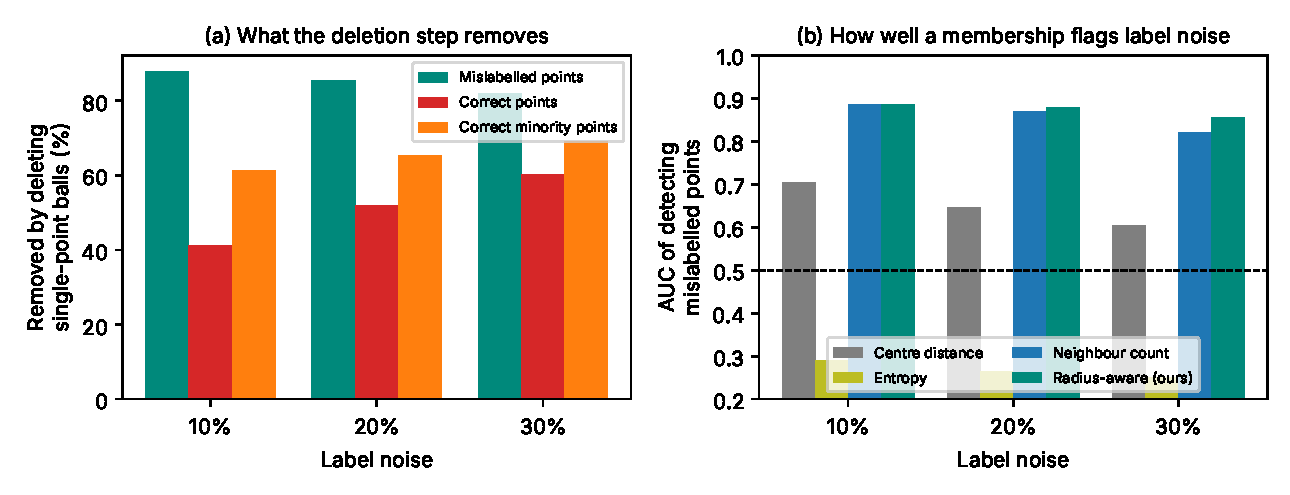
\includegraphics[width=\textwidth]{figures/diagnostics.pdf}
\caption{(a) Share of mislabelled, correctly labelled, and correctly labelled minority training samples that end up in single-sample balls and are deleted by GBLSTSVM. (b) Area under the ROC curve when a membership is used as a score for detecting mislabelled samples (each sample inherits the membership of its ball; all balls are kept). The dashed line is a random score. Averages over 21 datasets.}
\label{fig:diagnostics}
\end{figure}

A membership can only replace the deletion if it gives low values to mislabelled samples. Figure~\ref{fig:diagnostics}(b) treats each membership as a detector of mislabelled samples and reports the area under the ROC curve (AUC). The centre-distance membership used by existing fuzzy granular-ball SVMs reaches 0.70, 0.65 and 0.60 at 10\%, 20\% and 30\% noise. An entropy-based membership is below 0.5, because a mislabelled sample in its own ball has purity one and zero entropy. A plain count of agreeing neighbouring balls reaches 0.885, 0.868 and 0.821. The radius-aware membership proposed in the next section reaches 0.886, 0.877 and 0.854; its advantage over the plain count grows with the noise level.

%% ---------------------------------------------------------------------------
\section{Proposed model}
\label{sec:method}

\subsection{Radius-aware fuzzy membership}

Let $\{(c_i,r_i,y_i,n_i)\}_{i=1}^{m}$ be the balls generated from the training set, where $n_i$ is the number of samples in ball $i$. No ball is deleted. The \emph{surface gap} between two balls is
\begin{equation}
g_{ij}=\max\bigl(0,\ \lVert c_i-c_j\rVert-r_i-r_j\bigr),
\label{eq:gap}
\end{equation}
which is zero when the balls touch or overlap (Figure~\ref{fig:gap}). Let $N_k(i)$ be the $k$ balls with the smallest gap to ball $i$, and let $s_i=\max_{j\in N_k(i)}g_{ij}$ be the gap to the $k$-th of them. Ball $j\in N_k(i)$ votes with the weight
\begin{equation}
v_{ij}=n_j\exp\!\bigl(-(g_{ij}/s_i)^{2}\bigr),
\label{eq:vote}
\end{equation}
and the membership of ball $i$ is the share of the vote cast by balls of its own label, raised to a power $\gamma>0$:
\begin{equation}
m_i=\max\!\left(\epsilon,\ \Biggl(\frac{\sum_{j\in N_k(i)}v_{ij}\,[\,y_j=y_i\,]}{\sum_{j\in N_k(i)}v_{ij}}\Biggr)^{\!\gamma}\right),\qquad \epsilon=10^{-3}.
\label{eq:membership}
\end{equation}
Here $[\cdot]$ is one if the condition holds and zero otherwise.

\begin{figure}[t]
\centering
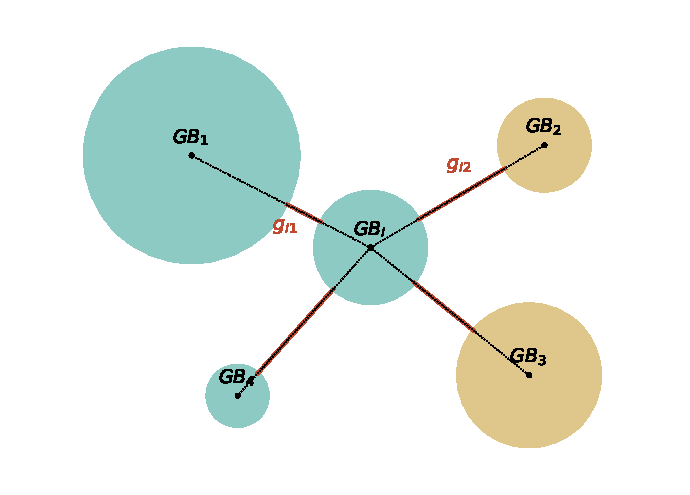
\includegraphics[width=0.5\textwidth]{figures/gap.pdf}
\caption{The surface gap. Ball $GB_1$ is large and almost touches $GB_i$, so it is a close neighbour although its centre (dotted line) is farther away than those of the other balls.}
\label{fig:gap}
\end{figure}

The three ingredients have the following purposes.
\begin{itemize}
\item \emph{Surface gap.} Balls differ strongly in size, from single samples to balls that cover a large part of a class. The centre distance treats a large ball as far away even when its surface is next to ball $i$. The gap \eqref{eq:gap} measures how far apart the regions covered by the two balls are.
\item \emph{Size and gap weights.} A neighbour that summarises many samples is stronger evidence than a single-sample ball, hence the factor $n_j$. The exponential factor lets touching balls count fully and lets the influence fade with the gap. Dividing by $s_i$ makes the weight independent of the scale of the data and adapts it to the local density, so that there is no bandwidth to tune.
\item \emph{Sharpness $\gamma$.} A value above one pushes the membership of balls with mixed neighbourhoods towards zero, a value below one flattens the membership.
\end{itemize}
A mislabelled sample that became a single-sample ball lies among balls of the other label, so its membership is close to $\epsilon$. A correct boundary sample has neighbours of both labels and receives an intermediate membership: it stays in the training set with reduced influence, instead of being deleted. A ball inside its class has membership one. The membership has two parameters, $k$ and $\gamma$; Section~\ref{sec:sensitivity} shows that the model is not sensitive to them.

\subsection{Linear \RF{}}

Let $C^{+}\in\R^{m_1\times d}$ and $C^{-}\in\R^{m_2\times d}$ hold the centres of the balls with label $+1$ and $-1$, $R^{+}$ and $R^{-}$ their radii, and $S^{+}=\operatorname{diag}(m_i)_{y_i=+1}$, $S^{-}=\operatorname{diag}(m_i)_{y_i=-1}$ their memberships. The two hyperplanes of the linear \RF{} are the solutions of
\begin{align}
\min_{w_1,b_1,\xi_1}\ & \frac{c_3}{2}\bigl(\lVert w_1\rVert^{2}+b_1^{2}\bigr)+\frac{1}{2}\lVert C^{+}w_1+eb_1\rVert^{2}+\frac{c_1}{2}\,\xi_1^{\top}S^{-}\xi_1 \nonumber\\
\text{s.t.}\ & -(C^{-}w_1+eb_1)+\xi_1=e+R^{-}, \label{eq:rf1}\\[4pt]
\min_{w_2,b_2,\xi_2}\ & \frac{c_4}{2}\bigl(\lVert w_2\rVert^{2}+b_2^{2}\bigr)+\frac{1}{2}\lVert C^{-}w_2+eb_2\rVert^{2}+\frac{c_2}{2}\,\xi_2^{\top}S^{+}\xi_2 \nonumber\\
\text{s.t.}\ & (C^{+}w_2+eb_2)+\xi_2=e+R^{+}. \label{eq:rf2}
\end{align}
In \eqref{eq:rf1}, the first term is the regulariser of LS-GBLSTSVM, the second keeps the first plane close to the balls of class $+1$, and the third penalises balls of class $-1$ that are not at distance one plus their radius from it. The penalty of each ball is multiplied by its membership, so a ball whose label is contradicted by its neighbours is allowed to lie on the wrong side at almost no cost. With $S^{\pm}=I$ and single-sample balls deleted, the problems reduce to LS-GBLSTSVM; with $c_3=c_4=0$ in addition, to GBLSTSVM.

Substituting the constraint of \eqref{eq:rf1} into the objective gives an unconstrained strictly convex quadratic in $z_1=[w_1^{\top}\ b_1]^{\top}$. With $H=[C^{+}\ \ e]$ and $G=[C^{-}\ \ e]$,
\[
L(z_1)=\frac{c_3}{2}\lVert z_1\rVert^{2}+\frac{1}{2}\lVert Hz_1\rVert^{2}+\frac{c_1}{2}\,(Gz_1+e+R^{-})^{\top}S^{-}(Gz_1+e+R^{-}),
\]
and setting $\nabla L=0$ yields
\begin{equation}
z_1=-\Bigl(G^{\top}S^{-}G+\tfrac{1}{c_1}H^{\top}H+\tfrac{c_3}{c_1}I\Bigr)^{-1}G^{\top}S^{-}(e+R^{-}).
\label{eq:sol1}
\end{equation}
In the same way,
\begin{equation}
z_2=\Bigl(H^{\top}S^{+}H+\tfrac{1}{c_2}G^{\top}G+\tfrac{c_4}{c_2}I\Bigr)^{-1}H^{\top}S^{+}(e+R^{+}).
\label{eq:sol2}
\end{equation}
Both matrices are of size $(d+1)\times(d+1)$ and positive definite for $c_3,c_4>0$, so the solution is unique. A new sample $x$ is assigned to the class of the nearer plane,
\begin{equation}
\operatorname{class}(x)=\argmin_{l\in\{1,2\}}\ \frac{\lvert w_l^{\top}x+b_l\rvert}{\lVert w_l\rVert},
\label{eq:decision}
\end{equation}
where $l=1$ stands for class $+1$ and $l=2$ for class $-1$. For imbalanced data, the diagonal entries that belong to the minority class can optionally be multiplied by the ratio of majority to minority samples; whether this is done is treated as a hyperparameter for every model in the experiments.

\subsection{Gaussian kernel \RF{}}

For the non-linear model we use the kernel-generated surfaces $K(x^{\top},D^{\top})u_l+b_l=0$, where $D=[C^{+};C^{-}]\in\R^{m\times d}$ holds all ball centres and $K(x,z)=\exp(-\mu\lVert x-z\rVert^{2})$. Since $D$ contains the $m$ ball centres rather than the $n$ training samples, the kernel matrix is small. The problems are \eqref{eq:rf1} and \eqref{eq:rf2} with $C^{+}$ and $C^{-}$ replaced by $K(C^{+},D^{\top})$ and $K(C^{-},D^{\top})$ and $w_l$ replaced by $u_l$, and the solutions are \eqref{eq:sol1} and \eqref{eq:sol2} with $H=[K(C^{+},D^{\top})\ \ e]$ and $G=[K(C^{-},D^{\top})\ \ e]$. The radii and the memberships are computed in the input space, as in the kernel GBLSTSVM \cite{tanveer2024gblstsvm}. The decision rule is \eqref{eq:decision} with $w_l^{\top}x$ replaced by $K(x^{\top},D^{\top})u_l$.

\subsection{Algorithm and complexity}

\begin{algorithm}[t]
\caption{Training of \RF{}}
\label{alg:rf}
\begin{algorithmic}[1]
\Require training set $T$; purity threshold; clusters per split; $k$, $\gamma$; $c_1,c_2,c_3,c_4$
\State Generate granular balls from $T$ by recursive $k$-means splitting until every ball reaches the purity threshold or holds one sample. Keep all balls.
\State Compute the surface gaps $g_{ij}$ by \eqref{eq:gap}.
\For{each ball $i$}
\State Find the $k$ balls with the smallest gap and compute $m_i$ by \eqref{eq:vote} and \eqref{eq:membership}.
\EndFor
\State Form $H$, $G$, $S^{+}$, $S^{-}$ (with the kernel map for the Gaussian model).
\State Compute $z_1$ and $z_2$ by \eqref{eq:sol1} and \eqref{eq:sol2}.
\Ensure $(w_1,b_1)$ and $(w_2,b_2)$; predict with \eqref{eq:decision}.
\end{algorithmic}
\end{algorithm}

Algorithm~\ref{alg:rf} summarises the training. With $m$ balls in $d$ dimensions, computing all gaps costs $O(m^{2}d)$ time and selecting the neighbours $O(m^{2})$. The linear model then needs $O(md^{2}+d^{3})$ for forming and solving the two systems, the same as LS-GBLSTSVM, and the kernel model $O(m^{3})$. Because all balls are kept, $m$ is larger than in GBLSTSVM; in exchange, no training sample is discarded. The quadratic cost of the gap computation is not a concern for the datasets used here. For very large data it can be reduced with a spatial index, which we leave for future work (Section~\ref{sec:discussion}).

%% ---------------------------------------------------------------------------
\section{Experiments}
\label{sec:experiments}

\subsection{Setup}
\label{sec:setup}

\paragraph{Datasets and noise} We use 35 binary datasets from the UCI \cite{uci} and KEEL \cite{keel} repositories (Table~\ref{tab:datasets}); the minority class is taken as the positive class. Each dataset is split at random into 70\% for training and 30\% for testing, stratified by class, and the features are standardised with the mean and standard deviation of the training part. Label noise is added by flipping the labels of 5\%, 10\%, 15\%, 20\% or 30\% of the training samples chosen at random; test labels are never changed. Every experiment is repeated over 10 random splits for the linear models and 5 for the Gaussian kernel, and the scores of a dataset are averaged over its splits. All models see exactly the same splits and the same flipped labels.

\begin{table}[!t]
\centering
\caption{The 35 UCI and KEEL benchmark datasets. IR is the imbalance ratio (majority size divided by minority size).}
\label{tab:datasets}
\footnotesize
\resizebox{\textwidth}{!}{%
\begin{tabular}{lrrr@{\hskip 18pt}lrrr}
\toprule
Dataset & Samples & Features & IR & Dataset & Samples & Features & IR \\
\midrule
abalone9-18 & 731 & 7 & 16.40 & led7digit-0-2-4-5-6-7-8-9\_vs\_1 & 443 & 7 & 10.97 \\
brwisconsin & 683 & 9 & 1.86 & monk2 & 601 & 7 & 1.92 \\
bupa or liver-disorders & 345 & 6 & 1.38 & monk3 & 554 & 6 & 1.01 \\
cleve & 297 & 13 & 1.17 & new-thyroid1 & 215 & 5 & 5.14 \\
ecoli-0-1-4-6\_vs\_5 & 280 & 6 & 13.00 & pima & 768 & 8 & 1.87 \\
ecoli-0-1-4-7\_vs\_2-3-5-6 & 336 & 7 & 10.59 & sonar & 208 & 60 & 1.14 \\
ecoli-0-1\_vs\_5 & 240 & 6 & 11.00 & transfusion & 748 & 4 & 3.20 \\
ecoli2 & 336 & 7 & 8.60 & vehicle 1 & 846 & 18 & 2.90 \\
ecoli3 & 336 & 7 & 8.60 & vehicle2 & 846 & 18 & 2.88 \\
ecoli4 & 336 & 7 & 15.80 & wdbc & 569 & 30 & 1.68 \\
fertility & 100 & 9 & 7.33 & wpbc & 194 & 33 & 3.22 \\
ger & 1000 & 24 & 2.33 & yeast-0-2-5-6\_vs\_3-7-8-9 & 1004 & 8 & 9.14 \\
glass2 & 214 & 9 & 11.59 & yeast-0-2-5-7-9\_vs\_3-6-8 & 1004 & 8 & 9.14 \\
glass4 & 214 & 9 & 15.46 & yeast-0-5-6-7-9\_vs\_4 & 528 & 8 & 9.35 \\
glass5 & 214 & 9 & 22.78 & yeast-2\_vs\_4 & 514 & 8 & 9.08 \\
haberman & 306 & 3 & 2.78 & yeast1vs7 & 459 & 8 & 14.30 \\
heart-stat & 270 & 13 & 1.25 & yeast3 & 1484 & 8 & 8.10 \\
iono & 351 & 33 & 1.79 &  &  &  &  \\
\bottomrule
\end{tabular}}
\end{table}


\paragraph{Models} \RF{} is compared with SVM \cite{cortes1995}, TSVM \cite{jayadeva2007}, GBSVM \cite{xia2022gbsvm}, LSTSVM \cite{kumar2009}, GBLSTSVM and LS-GBLSTSVM \cite{tanveer2024gblstsvm}, the baselines of \cite{tanveer2024gblstsvm}. All granular-ball models use the same ball generation with purity threshold 0.985; GBSVM, GBLSTSVM and LS-GBLSTSVM delete single-sample balls as in their original versions. The GBSVM problem \eqref{eq:gbsvm} is a second-order cone programme, and we solve it to optimality with an interior-point solver \cite{diamond2016,goulart2024} rather than with particle swarm optimisation.

\paragraph{Hyperparameters} The penalty parameters $c_1,c_2$ of LSTSVM and GBLSTSVM, $c_1=c_2$ and $c_3=c_4$ of LS-GBLSTSVM and \RF{}, and $C$ of SVM and GBSVM are taken from $\{10^{-3},10^{-2},\dots,10^{3}\}$, and those of TSVM from $\{2^{-5},\dots,2^{5}\}$. The number of clusters per split in the ball generation is taken from $\{2,\dots,6\}$ for the linear models and $\{2,4,6\}$ for the Gaussian kernel. The Gaussian kernel parameter is $\mu=q/d$ with $q\in\{0.25,1,4\}$. Every model can switch the class weighting for imbalanced data on or off. \RF{} has in addition $k\in\{5,10\}$ and $\gamma\in\{1,3\}$.

\paragraph{Two tuning protocols} The way the hyperparameters are chosen matters for the conclusions, so we report two protocols.
\begin{itemize}
\item \emph{Test-set tuning.} For each split, the reported score is the best test score over the grid. Several papers on fuzzy granular-ball SVMs select their hyperparameters in this way \cite{xia2024gbfsvm,lang2025gbftsvm}. The GBLSTSVM paper states that it uses five-fold cross-validation \cite{tanveer2024gblstsvm}; however, on the datasets we share with it, our test-tuned scores of GBLSTSVM are close to the published ones, while our cross-validated scores are several points lower, so we report both. It measures what a model can reach with ideal settings. It is optimistic, and it favours models with a larger grid, because the maximum over more settings can only be higher \cite{cawley2010}.
\item \emph{Cross-validation (CV) tuning.} For each split, the hyperparameters are chosen by five-fold cross-validation on the (noisy) training part, by the mean balanced accuracy over the folds, and the model with these settings is trained on the whole training part and scored once on the test part. This measures what a user obtains in practice, where test labels are not available for tuning.
\end{itemize}

\paragraph{Scores and tests} We report the accuracy (ACC) and the balanced accuracy (BACC, the mean of the recalls of the two classes), both in per cent. Following \cite{demsar2006}, models are compared by their average rank over the datasets, by the Friedman test with the Iman--Davenport correction \cite{iman1980}, and \RF{} is compared with each baseline by the Wilcoxon signed-rank test and by counting wins, ties and losses over the datasets.

\subsection{Linear kernel, test-set tuning}

Table~\ref{tab:lin-oracle} gives the average ACC and the average rank. \RF{} has the highest average ACC and the best average rank at every noise level, from 89.98\% on clean data to 88.10\% at 30\% noise, followed by LS-GBLSTSVM. Table~\ref{tab:lin-oracle-pair} shows that the difference to every baseline is significant at every noise level. The gain over LS-GBLSTSVM, the strongest baseline, is between 0.3 and 0.7 points with 23 to 28 wins out of 35 datasets ($p\le 0.002$); the gains over the other five baselines are between 1.2 and 5.1 points. From clean data to 30\% noise, \RF{} loses 1.9 points, LS-GBLSTSVM 2.1, GBLSTSVM 2.5, LSTSVM 2.9, SVM 3.1 and TSVM 3.3. The Friedman test rejects the hypothesis that all models perform equally in every setting (Table~\ref{tab:friedman}). The per-dataset scores at 0\% and 20\% noise are given in \ref{app:per-dataset}.

\begin{table}[!t]
\centering
\caption{Linear kernel, test-set tuning: average ACC (\%) and average rank over 35 datasets. Best value in each row in bold.}
\label{tab:lin-oracle}
\small
\resizebox{\textwidth}{!}{%
\begin{tabular}{llccccccc}
\toprule
 & Noise & SVM & TSVM & GBSVM & LSTSVM & GBLSTSVM & LS-GBLSTSVM & \textbf{RF-GBLSTSVM} \\
\midrule
Average ACC & 0\% & 88.53 & 88.59 & 84.96 & 88.21 & 88.08 & 89.50 & \textbf{89.98} \\
 & 5\% & 87.91 & 88.61 & 85.11 & 88.05 & 87.98 & 89.30 & \textbf{89.83} \\
 & 10\% & 87.08 & 88.23 & 84.87 & 87.56 & 87.93 & 89.20 & \textbf{89.53} \\
 & 15\% & 86.47 & 87.59 & 84.58 & 87.14 & 87.52 & 88.87 & \textbf{89.33} \\
 & 20\% & 86.17 & 87.07 & 83.97 & 86.79 & 87.06 & 88.66 & \textbf{89.08} \\
 & 30\% & 85.39 & 85.33 & 83.09 & 85.27 & 85.56 & 87.41 & \textbf{88.10} \\
\midrule
Average rank & 0\% & 4.94 & 4.27 & 5.40 & 5.31 & 4.16 & 2.46 & \textbf{1.46} \\
 & 5\% & 5.44 & 3.96 & 5.30 & 5.51 & 3.86 & 2.43 & \textbf{1.50} \\
 & 10\% & 5.56 & 4.20 & 5.27 & 5.47 & 3.84 & 2.14 & \textbf{1.51} \\
 & 15\% & 5.67 & 4.34 & 5.57 & 5.31 & 3.49 & 2.26 & \textbf{1.36} \\
 & 20\% & 5.66 & 4.37 & 5.70 & 5.00 & 3.61 & 2.21 & \textbf{1.44} \\
 & 30\% & 5.43 & 4.70 & 5.90 & 4.69 & 3.59 & 2.29 & \textbf{1.41} \\
\bottomrule
\end{tabular}}
\end{table}

\begin{table}[!t]
\centering
\caption{RF-GBLSTSVM against each baseline, linear kernel, test-set tuning: mean difference in ACC (percentage points), [win, tie, loss] over the 35 datasets and, in parentheses, the $p$-value of the Wilcoxon signed-rank test.}
\label{tab:lin-oracle-pair}
\footnotesize
\resizebox{\textwidth}{!}{%
\begin{tabular}{lcccccc}
\toprule
Baseline & 0\% & 5\% & 10\% & 15\% & 20\% & 30\% \\
\midrule
SVM & \shortstack{+1.45 [34, 0, 1]\\($<$0.001)} & \shortstack{+1.92 [34, 1, 0]\\($<$0.001)} & \shortstack{+2.45 [34, 0, 1]\\($<$0.001)} & \shortstack{+2.85 [35, 0, 0]\\($<$0.001)} & \shortstack{+2.91 [35, 0, 0]\\($<$0.001)} & \shortstack{+2.71 [34, 1, 0]\\($<$0.001)} \\[4pt]
TSVM & \shortstack{+1.39 [33, 0, 2]\\($<$0.001)} & \shortstack{+1.22 [33, 0, 2]\\($<$0.001)} & \shortstack{+1.30 [34, 0, 1]\\($<$0.001)} & \shortstack{+1.73 [34, 0, 1]\\($<$0.001)} & \shortstack{+2.01 [34, 0, 1]\\($<$0.001)} & \shortstack{+2.76 [33, 1, 1]\\($<$0.001)} \\[4pt]
GBSVM & \shortstack{+5.03 [33, 0, 2]\\($<$0.001)} & \shortstack{+4.72 [32, 1, 2]\\($<$0.001)} & \shortstack{+4.66 [33, 1, 1]\\($<$0.001)} & \shortstack{+4.75 [35, 0, 0]\\($<$0.001)} & \shortstack{+5.11 [34, 0, 1]\\($<$0.001)} & \shortstack{+5.01 [34, 1, 0]\\($<$0.001)} \\[4pt]
LSTSVM & \shortstack{+1.77 [35, 0, 0]\\($<$0.001)} & \shortstack{+1.78 [35, 0, 0]\\($<$0.001)} & \shortstack{+1.98 [35, 0, 0]\\($<$0.001)} & \shortstack{+2.19 [35, 0, 0]\\($<$0.001)} & \shortstack{+2.28 [35, 0, 0]\\($<$0.001)} & \shortstack{+2.83 [34, 1, 0]\\($<$0.001)} \\[4pt]
GBLSTSVM & \shortstack{+1.90 [32, 0, 3]\\($<$0.001)} & \shortstack{+1.85 [30, 2, 3]\\($<$0.001)} & \shortstack{+1.60 [29, 2, 4]\\($<$0.001)} & \shortstack{+1.80 [31, 0, 4]\\($<$0.001)} & \shortstack{+2.01 [31, 0, 4]\\($<$0.001)} & \shortstack{+2.54 [29, 2, 4]\\($<$0.001)} \\[4pt]
LS-GBLSTSVM & \shortstack{+0.48 [27, 0, 8]\\($<$0.001)} & \shortstack{+0.52 [25, 3, 7]\\($<$0.001)} & \shortstack{+0.33 [23, 5, 7]\\(0.002)} & \shortstack{+0.46 [27, 1, 7]\\($<$0.001)} & \shortstack{+0.42 [25, 1, 9]\\(0.001)} & \shortstack{+0.69 [28, 1, 6]\\($<$0.001)} \\[4pt]
\bottomrule
\end{tabular}}
\end{table}


\subsection{Linear kernel, CV tuning}

Tables~\ref{tab:lin-cv-acc} to \ref{tab:lin-cv-bacc-pair} give the results when the hyperparameters are chosen by cross-validation on the training part. All scores are clearly lower than under test-set tuning, by 5 to 20 points for most models, and the ranking changes.

\emph{Accuracy.} On clean data, SVM is the best model (83.2\%) and is significantly ahead of \RF{} (81.4\%, $p=0.004$); \RF{}, LS-GBLSTSVM, TSVM and LSTSVM are within about one point of each other. With label noise the picture turns. From 5\% noise upwards \RF{} has the best average rank, and from 15\% upwards the best average ACC. At 20\% noise it reaches 77.9\%, against 75.1\% for LS-GBLSTSVM, 74.4\% for SVM and 73.5\% for LSTSVM. Compared with LS-GBLSTSVM, \RF{} is level up to 10\% noise (differences below half a point, not significant) and ahead by 1.3, 2.8 and 3.7 points at 15\%, 20\% and 30\% ($p=0.041$, $0.003$, $0.004$). Compared with GBLSTSVM it is ahead by 3.2 to 9.7 points at every noise level.

\emph{Balanced accuracy.} BACC is the harder score for the granular-ball models, because many of the datasets are strongly imbalanced. SVM has the highest average BACC up to 15\% noise, and SVM, LSTSVM and TSVM are significantly ahead of \RF{} on clean data (by 2.3 to 3.0 points). \RF{} catches up as the noise grows: at 20\% and 30\% it has the highest average BACC (75.3\% and 70.3\%), although its differences to SVM at these levels are not significant. Among the granular-ball models \RF{} is the best at every noise level; it is ahead of GBLSTSVM by 3.0 to 6.6 points (always significant) and of LS-GBLSTSVM by 0.3 to 2.4 points (significant at 20\% and 30\%).

Figure~\ref{fig:noise-linear} shows both protocols side by side.

\begin{table}[!t]
\centering
\caption{Linear kernel, cross-validated tuning: average ACC (\%) and average rank over 35 datasets.}
\label{tab:lin-cv-acc}
\small
\resizebox{\textwidth}{!}{%
\begin{tabular}{llccccccc}
\toprule
 & Noise & SVM & TSVM & GBSVM & LSTSVM & GBLSTSVM & LS-GBLSTSVM & \textbf{RF-GBLSTSVM} \\
\midrule
Average ACC & 0\% & \textbf{83.22} & 81.92 & 68.56 & 81.01 & 78.23 & 81.45 & 81.40 \\
 & 5\% & 79.76 & 79.11 & 70.26 & 79.41 & 77.77 & \textbf{81.10} & 81.02 \\
 & 10\% & 77.82 & 77.74 & 68.74 & 77.47 & 76.40 & \textbf{80.01} & 79.60 \\
 & 15\% & 75.98 & 74.99 & 64.15 & 75.82 & 74.32 & 77.47 & \textbf{78.77} \\
 & 20\% & 74.42 & 73.14 & 61.26 & 73.46 & 70.49 & 75.13 & \textbf{77.92} \\
 & 30\% & 72.20 & 65.52 & 52.50 & 66.05 & 64.06 & 70.03 & \textbf{73.76} \\
\midrule
Average rank & 0\% & \textbf{2.73} & 3.34 & 5.69 & 3.80 & 4.93 & 3.64 & 3.87 \\
 & 5\% & 3.79 & 4.06 & 5.63 & 3.80 & 5.17 & 2.87 & \textbf{2.69} \\
 & 10\% & 3.76 & 3.70 & 5.69 & 4.03 & 4.99 & 3.23 & \textbf{2.61} \\
 & 15\% & 3.84 & 4.19 & 5.46 & 3.76 & 4.84 & 3.29 & \textbf{2.63} \\
 & 20\% & 3.47 & 4.06 & 5.89 & 3.83 & 5.14 & 3.56 & \textbf{2.06} \\
 & 30\% & 2.56 & 4.36 & 5.94 & 4.59 & 4.91 & 3.51 & \textbf{2.13} \\
\bottomrule
\end{tabular}}
\end{table}

\begin{table}[!t]
\centering
\caption{RF-GBLSTSVM against each baseline, linear kernel, cross-validated tuning: mean difference in ACC (percentage points), [win, tie, loss] over the 35 datasets and, in parentheses, the $p$-value of the Wilcoxon signed-rank test.}
\label{tab:lin-cv-acc-pair}
\footnotesize
\resizebox{\textwidth}{!}{%
\begin{tabular}{lcccccc}
\toprule
Baseline & 0\% & 5\% & 10\% & 15\% & 20\% & 30\% \\
\midrule
SVM & \shortstack{-1.82 [8, 1, 26]\\(0.004)} & \shortstack{+1.26 [22, 2, 11]\\(0.036)} & \shortstack{+1.79 [19, 1, 15]\\(0.106)} & \shortstack{+2.80 [21, 0, 14]\\(0.008)} & \shortstack{+3.50 [25, 0, 10]\\(0.008)} & \shortstack{+1.56 [19, 1, 15]\\(0.309)} \\[4pt]
TSVM & \shortstack{-0.52 [14, 0, 21]\\(0.235)} & \shortstack{+1.91 [27, 0, 8]\\($<$0.001)} & \shortstack{+1.87 [26, 0, 9]\\($<$0.001)} & \shortstack{+3.78 [26, 0, 9]\\($<$0.001)} & \shortstack{+4.78 [30, 0, 5]\\($<$0.001)} & \shortstack{+8.25 [31, 0, 4]\\($<$0.001)} \\[4pt]
GBSVM & \shortstack{+12.84 [29, 0, 6]\\($<$0.001)} & \shortstack{+10.76 [29, 0, 6]\\($<$0.001)} & \shortstack{+10.86 [30, 0, 5]\\($<$0.001)} & \shortstack{+14.63 [31, 0, 4]\\($<$0.001)} & \shortstack{+16.67 [32, 0, 3]\\($<$0.001)} & \shortstack{+21.26 [30, 0, 5]\\($<$0.001)} \\[4pt]
LSTSVM & \shortstack{+0.39 [16, 0, 19]\\(0.974)} & \shortstack{+1.62 [24, 0, 11]\\(0.007)} & \shortstack{+2.13 [26, 0, 9]\\(0.002)} & \shortstack{+2.95 [22, 2, 11]\\(0.005)} & \shortstack{+4.47 [29, 0, 6]\\($<$0.001)} & \shortstack{+7.72 [33, 0, 2]\\($<$0.001)} \\[4pt]
GBLSTSVM & \shortstack{+3.17 [25, 0, 10]\\(0.005)} & \shortstack{+3.25 [29, 2, 4]\\($<$0.001)} & \shortstack{+3.20 [27, 0, 8]\\(0.005)} & \shortstack{+4.46 [28, 0, 7]\\($<$0.001)} & \shortstack{+7.44 [30, 0, 5]\\($<$0.001)} & \shortstack{+9.70 [29, 0, 6]\\($<$0.001)} \\[4pt]
LS-GBLSTSVM & \shortstack{-0.05 [17, 0, 18]\\(1.000)} & \shortstack{-0.07 [18, 0, 17]\\(0.376)} & \shortstack{-0.41 [25, 0, 10]\\(0.085)} & \shortstack{+1.30 [24, 0, 11]\\(0.041)} & \shortstack{+2.79 [27, 0, 8]\\(0.003)} & \shortstack{+3.73 [28, 0, 7]\\(0.004)} \\[4pt]
\bottomrule
\end{tabular}}
\end{table}

\begin{table}[!t]
\centering
\caption{Linear kernel, cross-validated tuning: average balanced accuracy (BACC, \%) and average rank over 35 datasets.}
\label{tab:lin-cv-bacc}
\small
\resizebox{\textwidth}{!}{%
\begin{tabular}{llccccccc}
\toprule
 & Noise & SVM & TSVM & GBSVM & LSTSVM & GBLSTSVM & LS-GBLSTSVM & \textbf{RF-GBLSTSVM} \\
\midrule
Average BACC & 0\% & \textbf{81.01} & 80.32 & 66.99 & 80.45 & 74.17 & 76.93 & 78.03 \\
 & 5\% & \textbf{79.79} & 78.68 & 69.85 & 79.20 & 75.11 & 77.83 & 78.14 \\
 & 10\% & \textbf{78.75} & 77.87 & 69.24 & 77.93 & 74.15 & 76.48 & 77.50 \\
 & 15\% & \textbf{76.85} & 75.46 & 67.44 & 76.37 & 72.33 & 74.59 & 75.37 \\
 & 20\% & 75.21 & 74.53 & 65.56 & 74.32 & 69.99 & 72.85 & \textbf{75.26} \\
 & 30\% & 69.72 & 68.56 & 59.65 & 68.69 & 63.68 & 67.96 & \textbf{70.27} \\
\midrule
Average rank & 0\% & \textbf{2.31} & 2.64 & 6.31 & 2.77 & 5.49 & 4.51 & 3.96 \\
 & 5\% & \textbf{2.67} & 3.57 & 6.00 & 2.99 & 5.40 & 3.74 & 3.63 \\
 & 10\% & \textbf{2.80} & 3.11 & 5.87 & 3.04 & 5.40 & 4.23 & 3.54 \\
 & 15\% & \textbf{2.60} & 3.71 & 5.83 & 2.71 & 5.26 & 4.09 & 3.80 \\
 & 20\% & \textbf{2.66} & 3.11 & 6.11 & 3.39 & 5.51 & 4.40 & 2.81 \\
 & 30\% & 3.14 & 3.37 & 5.71 & 3.63 & 5.20 & 4.17 & \textbf{2.77} \\
\bottomrule
\end{tabular}}
\end{table}

\begin{table}[!t]
\centering
\caption{RF-GBLSTSVM against each baseline, linear kernel, cross-validated tuning: mean difference in BACC (percentage points), [win, tie, loss] over the 35 datasets and, in parentheses, the $p$-value of the Wilcoxon signed-rank test.}
\label{tab:lin-cv-bacc-pair}
\footnotesize
\resizebox{\textwidth}{!}{%
\begin{tabular}{lcccccc}
\toprule
Baseline & 0\% & 5\% & 10\% & 15\% & 20\% & 30\% \\
\midrule
SVM & \shortstack{-2.97 [6, 0, 29]\\($<$0.001)} & \shortstack{-1.65 [14, 0, 21]\\(0.009)} & \shortstack{-1.25 [13, 0, 22]\\(0.033)} & \shortstack{-1.48 [11, 0, 24]\\(0.015)} & \shortstack{+0.04 [17, 0, 18]\\(0.909)} & \shortstack{+0.55 [20, 0, 15]\\(0.413)} \\[4pt]
TSVM & \shortstack{-2.29 [12, 0, 23]\\(0.003)} & \shortstack{-0.54 [16, 0, 19]\\(0.432)} & \shortstack{-0.38 [13, 0, 22]\\(0.326)} & \shortstack{-0.09 [17, 0, 18]\\(0.961)} & \shortstack{+0.72 [19, 0, 16]\\(0.291)} & \shortstack{+1.71 [21, 0, 14]\\(0.055)} \\[4pt]
GBSVM & \shortstack{+11.04 [32, 0, 3]\\($<$0.001)} & \shortstack{+8.29 [30, 0, 5]\\($<$0.001)} & \shortstack{+8.26 [29, 0, 6]\\($<$0.001)} & \shortstack{+7.93 [29, 0, 6]\\($<$0.001)} & \shortstack{+9.70 [33, 0, 2]\\($<$0.001)} & \shortstack{+10.62 [28, 0, 7]\\($<$0.001)} \\[4pt]
LSTSVM & \shortstack{-2.41 [8, 1, 26]\\($<$0.001)} & \shortstack{-1.06 [14, 0, 21]\\(0.036)} & \shortstack{-0.43 [14, 0, 21]\\(0.110)} & \shortstack{-1.00 [10, 0, 25]\\(0.038)} & \shortstack{+0.94 [22, 1, 12]\\(0.122)} & \shortstack{+1.58 [24, 0, 11]\\(0.015)} \\[4pt]
GBLSTSVM & \shortstack{+3.86 [28, 0, 7]\\($<$0.001)} & \shortstack{+3.03 [27, 0, 8]\\($<$0.001)} & \shortstack{+3.35 [29, 0, 6]\\($<$0.001)} & \shortstack{+3.04 [26, 0, 9]\\(0.001)} & \shortstack{+5.27 [28, 0, 7]\\($<$0.001)} & \shortstack{+6.59 [29, 0, 6]\\($<$0.001)} \\[4pt]
LS-GBLSTSVM & \shortstack{+1.10 [20, 0, 15]\\(0.238)} & \shortstack{+0.31 [17, 0, 18]\\(0.896)} & \shortstack{+1.02 [23, 0, 12]\\(0.057)} & \shortstack{+0.78 [19, 0, 16]\\(0.326)} & \shortstack{+2.41 [27, 0, 8]\\(0.001)} & \shortstack{+2.30 [26, 0, 9]\\(0.008)} \\[4pt]
\bottomrule
\end{tabular}}
\end{table}


\begin{figure}[t]
\centering
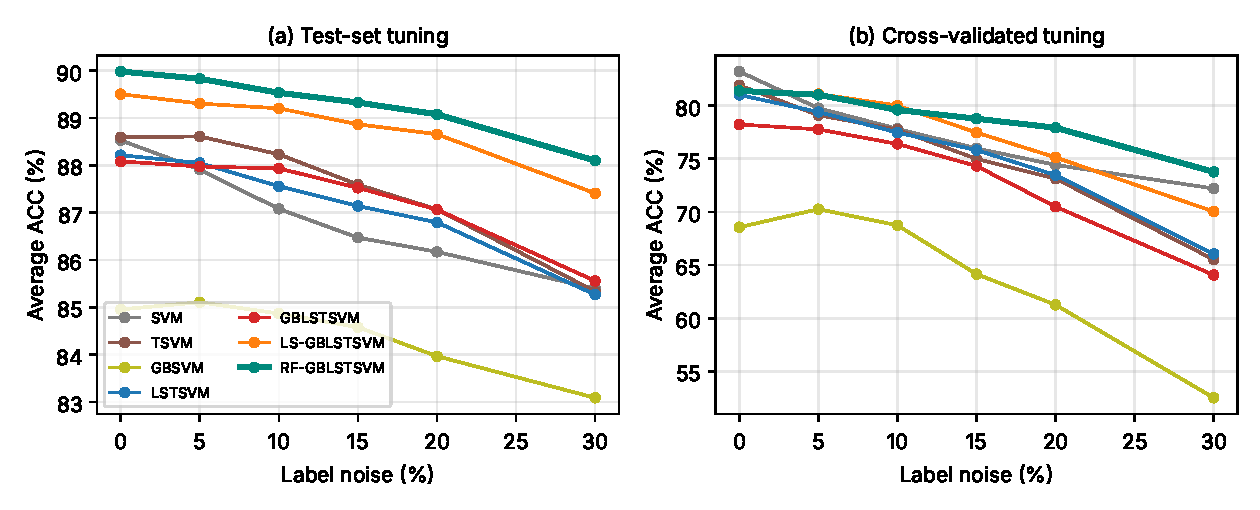
\includegraphics[width=\textwidth]{figures/noise_linear.pdf}
\caption{Linear kernel: average score over 35 datasets against the label noise level, under test-set tuning and under CV tuning.}
\label{fig:noise-linear}
\end{figure}

\subsection{Gaussian kernel}

Tables~\ref{tab:ker-oracle} to \ref{tab:ker-cv-bacc-pair} and Figure~\ref{fig:noise-kernel} give the results with the Gaussian kernel at 0\%, 10\% and 20\% noise. Under test-set tuning, \RF{} is again first at every noise level (91.9\%, 91.1\% and 90.2\% ACC) with an average rank between 1.5 and 1.7, and it is significantly better than each of the six baselines; the gain over LS-GBLSTSVM is 0.5 to 1.0 points. Under CV tuning the point-based models are stronger than in the linear case. TSVM and SVM have the highest ACC, and SVM has the highest BACC at every noise level. \RF{} has the second-highest BACC (81.9\%, 78.8\% and 73.9\%). It is the best of the five twin and granular-ball models, significantly ahead of GBLSTSVM and TSVM at every level, of LS-GBLSTSVM at 0\% and 10\%, and of LSTSVM at 10\% and 20\%, and it is behind SVM by 0.8 to 1.8 points (significant at 10\% and 20\%).

\begin{table}[!t]
\centering
\caption{Gaussian kernel, test-set tuning: average ACC (\%) and average rank over 35 datasets.}
\label{tab:ker-oracle}
\small
\resizebox{\textwidth}{!}{%
\begin{tabular}{llccccccc}
\toprule
 & Noise & SVM & TSVM & GBSVM & LSTSVM & GBLSTSVM & LS-GBLSTSVM & \textbf{RF-GBLSTSVM} \\
\midrule
Average ACC & 0\% & 90.77 & 90.74 & 78.97 & 90.76 & 90.31 & 90.88 & \textbf{91.87} \\
 & 10\% & 89.94 & 89.10 & 80.92 & 88.90 & 89.79 & 90.45 & \textbf{91.06} \\
 & 20\% & 88.64 & 86.53 & 80.65 & 86.75 & 88.81 & 89.72 & \textbf{90.18} \\
\midrule
Average rank & 0\% & 4.63 & 4.17 & 6.90 & 3.87 & 3.84 & 3.01 & \textbf{1.57} \\
 & 10\% & 3.84 & 4.56 & 6.77 & 5.09 & 3.54 & 2.50 & \textbf{1.70} \\
 & 20\% & 3.86 & 5.29 & 6.59 & 5.10 & 3.54 & 2.14 & \textbf{1.49} \\
\bottomrule
\end{tabular}}
\end{table}

\begin{table}[!t]
\centering
\caption{RF-GBLSTSVM against each baseline, Gaussian kernel, test-set tuning: mean difference in ACC (percentage points), [win, tie, loss] over the 35 datasets and, in parentheses, the $p$-value of the Wilcoxon signed-rank test.}
\label{tab:ker-oracle-pair}
\footnotesize
\resizebox{\textwidth}{!}{%
\begin{tabular}{lccc}
\toprule
Baseline & 0\% & 10\% & 20\% \\
\midrule
SVM & \shortstack{+1.09 [32, 0, 3]\\($<$0.001)} & \shortstack{+1.12 [31, 1, 3]\\($<$0.001)} & \shortstack{+1.55 [32, 1, 2]\\($<$0.001)} \\[4pt]
TSVM & \shortstack{+1.13 [31, 0, 4]\\($<$0.001)} & \shortstack{+1.95 [30, 0, 5]\\($<$0.001)} & \shortstack{+3.66 [34, 0, 1]\\($<$0.001)} \\[4pt]
GBSVM & \shortstack{+12.89 [35, 0, 0]\\($<$0.001)} & \shortstack{+10.13 [35, 0, 0]\\($<$0.001)} & \shortstack{+9.53 [35, 0, 0]\\($<$0.001)} \\[4pt]
LSTSVM & \shortstack{+1.10 [30, 1, 4]\\($<$0.001)} & \shortstack{+2.16 [34, 0, 1]\\($<$0.001)} & \shortstack{+3.44 [33, 2, 0]\\($<$0.001)} \\[4pt]
GBLSTSVM & \shortstack{+1.55 [31, 2, 2]\\($<$0.001)} & \shortstack{+1.27 [29, 3, 3]\\($<$0.001)} & \shortstack{+1.38 [30, 1, 4]\\($<$0.001)} \\[4pt]
LS-GBLSTSVM & \shortstack{+0.99 [28, 3, 4]\\($<$0.001)} & \shortstack{+0.61 [19, 11, 5]\\(0.006)} & \shortstack{+0.47 [25, 4, 6]\\(0.006)} \\[4pt]
\bottomrule
\end{tabular}}
\end{table}

\begin{table}[!t]
\centering
\caption{Gaussian kernel, cross-validated tuning: average ACC (\%) and average rank over 35 datasets.}
\label{tab:ker-cv-acc}
\small
\resizebox{\textwidth}{!}{%
\begin{tabular}{llccccccc}
\toprule
 & Noise & SVM & TSVM & GBSVM & LSTSVM & GBLSTSVM & LS-GBLSTSVM & \textbf{RF-GBLSTSVM} \\
\midrule
Average ACC & 0\% & 86.31 & \textbf{88.29} & 61.53 & 84.01 & 80.54 & 82.43 & 85.11 \\
 & 10\% & 82.19 & \textbf{83.43} & 63.26 & 78.27 & 78.09 & 78.43 & 80.08 \\
 & 20\% & \textbf{76.64} & 76.20 & 56.31 & 71.89 & 72.20 & 72.54 & 74.13 \\
\midrule
Average rank & 0\% & 2.79 & \textbf{1.81} & 6.01 & 3.84 & 5.30 & 4.59 & 3.66 \\
 & 10\% & 2.60 & \textbf{2.54} & 6.23 & 4.49 & 4.51 & 3.97 & 3.66 \\
 & 20\% & \textbf{2.43} & 3.24 & 6.09 & 4.41 & 4.51 & 3.74 & 3.57 \\
\bottomrule
\end{tabular}}
\end{table}

\begin{table}[!t]
\centering
\caption{Gaussian kernel, cross-validated tuning: average BACC (\%) and average rank over 35 datasets.}
\label{tab:ker-cv-bacc}
\small
\resizebox{\textwidth}{!}{%
\begin{tabular}{llccccccc}
\toprule
 & Noise & SVM & TSVM & GBSVM & LSTSVM & GBLSTSVM & LS-GBLSTSVM & \textbf{RF-GBLSTSVM} \\
\midrule
Average BACC & 0\% & \textbf{82.63} & 78.37 & 53.20 & 81.26 & 77.58 & 78.80 & 81.86 \\
 & 10\% & \textbf{80.25} & 77.23 & 61.83 & 74.90 & 74.21 & 76.30 & 78.82 \\
 & 20\% & \textbf{75.71} & 71.08 & 57.46 & 69.52 & 70.28 & 72.33 & 73.90 \\
\midrule
Average rank & 0\% & \textbf{2.33} & 4.30 & 6.80 & 3.00 & 4.80 & 3.97 & 2.80 \\
 & 10\% & \textbf{1.97} & 3.54 & 6.40 & 4.83 & 4.67 & 3.59 & 3.00 \\
 & 20\% & \textbf{1.83} & 4.09 & 6.51 & 4.69 & 4.51 & 3.40 & 2.97 \\
\bottomrule
\end{tabular}}
\end{table}

\begin{table}[!t]
\centering
\caption{RF-GBLSTSVM against each baseline, Gaussian kernel, cross-validated tuning: mean difference in BACC (percentage points), [win, tie, loss] over the 35 datasets and, in parentheses, the $p$-value of the Wilcoxon signed-rank test.}
\label{tab:ker-cv-bacc-pair}
\footnotesize
\resizebox{\textwidth}{!}{%
\begin{tabular}{lccc}
\toprule
Baseline & 0\% & 10\% & 20\% \\
\midrule
SVM & \shortstack{-0.77 [14, 0, 21]\\(0.055)} & \shortstack{-1.43 [7, 0, 28]\\(0.013)} & \shortstack{-1.81 [7, 0, 28]\\(0.001)} \\[4pt]
TSVM & \shortstack{+3.49 [26, 0, 9]\\(0.003)} & \shortstack{+1.59 [23, 0, 12]\\(0.049)} & \shortstack{+2.81 [24, 0, 11]\\($<$0.001)} \\[4pt]
GBSVM & \shortstack{+28.66 [35, 0, 0]\\($<$0.001)} & \shortstack{+16.98 [33, 0, 2]\\($<$0.001)} & \shortstack{+16.44 [33, 0, 2]\\($<$0.001)} \\[4pt]
LSTSVM & \shortstack{+0.60 [20, 0, 15]\\(0.385)} & \shortstack{+3.92 [26, 0, 9]\\($<$0.001)} & \shortstack{+4.38 [30, 0, 5]\\($<$0.001)} \\[4pt]
GBLSTSVM & \shortstack{+4.27 [27, 2, 6]\\($<$0.001)} & \shortstack{+4.61 [30, 0, 5]\\($<$0.001)} & \shortstack{+3.61 [29, 0, 6]\\($<$0.001)} \\[4pt]
LS-GBLSTSVM & \shortstack{+3.06 [24, 0, 11]\\(0.001)} & \shortstack{+2.52 [21, 0, 14]\\(0.008)} & \shortstack{+1.57 [18, 0, 17]\\(0.219)} \\[4pt]
\bottomrule
\end{tabular}}
\end{table}

\begin{table}[!t]
\centering
\caption{Friedman test over the seven models. $\chi^2_F$ has 6 degrees of freedom; $F_F$ is the Iman--Davenport statistic. Every $p$-value is below $10^{-6}$, so the hypothesis that all models perform equally is rejected in every setting.}
\label{tab:friedman}
\small
\begin{tabular}{lllccc}
\toprule
Kernel & Tuning & Score & Noise & $\chi^2_F$ & $F_F$ \\
\midrule
Linear & Test-set & ACC & 0\% & 101.41 & 31.75 \\
Linear & Test-set & ACC & 10\% & 119.24 & 44.67 \\
Linear & Test-set & ACC & 20\% & 124.88 & 49.88 \\
Linear & Test-set & BACC & 0\% & 92.49 & 26.76 \\
Linear & Test-set & BACC & 10\% & 114.01 & 40.38 \\
Linear & Test-set & BACC & 20\% & 126.58 & 51.60 \\
Linear & CV & ACC & 0\% & 44.52 & 9.15 \\
Linear & CV & ACC & 10\% & 48.59 & 10.23 \\
Linear & CV & ACC & 20\% & 68.59 & 16.49 \\
Linear & CV & BACC & 0\% & 105.17 & 34.11 \\
Linear & CV & BACC & 10\% & 66.48 & 15.75 \\
Linear & CV & BACC & 20\% & 84.71 & 22.99 \\
Gaussian & Test-set & ACC & 0\% & 118.09 & 43.68 \\
Gaussian & Test-set & ACC & 10\% & 127.08 & 52.10 \\
Gaussian & Test-set & ACC & 20\% & 146.62 & 78.65 \\
Gaussian & Test-set & BACC & 0\% & 127.40 & 52.44 \\
Gaussian & Test-set & BACC & 10\% & 124.44 & 49.45 \\
Gaussian & Test-set & BACC & 20\% & 158.23 & 103.93 \\
Gaussian & CV & ACC & 0\% & 93.63 & 27.36 \\
Gaussian & CV & ACC & 10\% & 72.51 & 17.93 \\
Gaussian & CV & ACC & 20\% & 60.59 & 13.79 \\
Gaussian & CV & BACC & 0\% & 103.53 & 33.06 \\
Gaussian & CV & BACC & 10\% & 92.95 & 27.00 \\
Gaussian & CV & BACC & 20\% & 98.98 & 30.31 \\
\bottomrule
\end{tabular}
\end{table}


\begin{figure}[t]
\centering
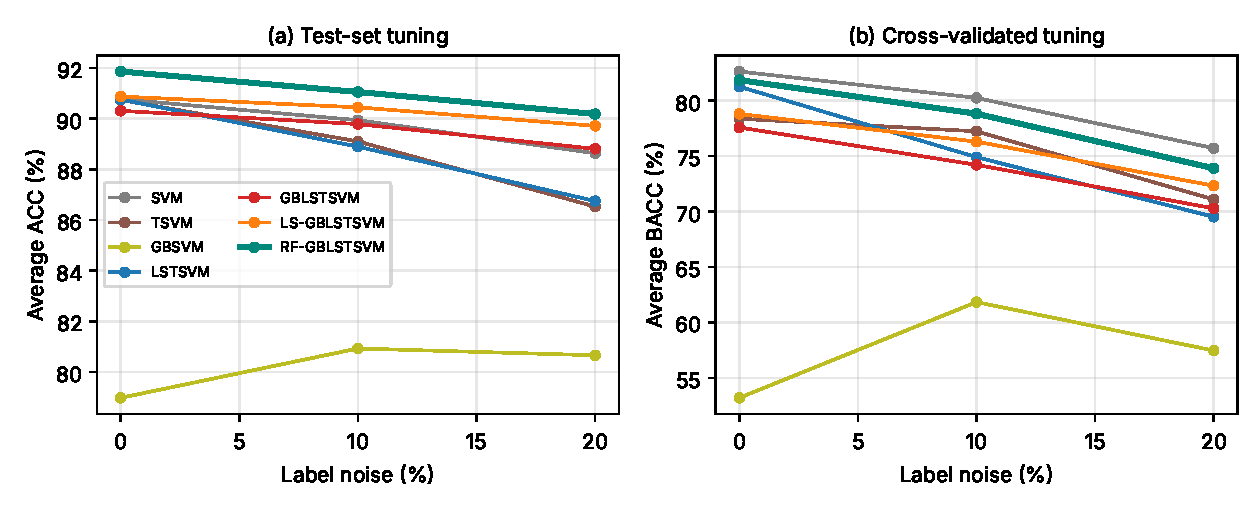
\includegraphics[width=\textwidth]{figures/noise_kernel.pdf}
\caption{Gaussian kernel: average score over 35 datasets against the label noise level, under test-set tuning and under CV tuning.}
\label{fig:noise-kernel}
\end{figure}

\subsection{Ablation}

\RF{} differs from GBLSTSVM in three components: single-sample balls are kept, the error terms are weighted by the radius-aware membership, and the regularisation term is added. Table~\ref{tab:ablation} shows the linear model with each combination that we ran. Three observations can be made. First, keeping the balls without a membership is not enough. Added to GBLSTSVM it helps by 0.3 to 1.5 points, but added to LS-GBLSTSVM it lowers the accuracy under both protocols (for example from 75.1\% to 73.8\% at 20\% noise under CV tuning), because the mislabelled single-sample balls return to the training set with full weight. Second, the membership repairs this: with the membership on top, the model gains 4.1 points at 20\% noise and 4.8 points at 30\% under CV tuning, and ends above LS-GBLSTSVM. Third, the regularisation term matters most under CV tuning, where it adds about 3 to 7 points to the model with kept balls and membership. The full model is the best row under test-set tuning at every noise level and under CV tuning at 20\% and 30\% noise; on clean data and at 10\% noise under CV tuning it is level with LS-GBLSTSVM.

\begin{table}[!t]
\centering
\caption{Ablation of the three components (linear kernel, average ACC in \% over 35 datasets). Keep: single-point balls are retained. Fuzzy: radius-aware membership. Reg.: regularisation term of LS-GBLSTSVM. The first row is GBLSTSVM, the fourth is LS-GBLSTSVM and the last is the proposed RF-GBLSTSVM.}
\label{tab:ablation}
\small
\resizebox{\textwidth}{!}{%
\begin{tabular}{ccccccccccc}
\toprule
 & & & \multicolumn{4}{c}{Test-set tuning} & \multicolumn{4}{c}{CV tuning} \\ \cmidrule(lr){4-7}\cmidrule(lr){8-11}
Keep & Fuzzy & Reg. & 0\% & 10\% & 20\% & 30\% & 0\% & 10\% & 20\% & 30\% \\
\midrule
 &  &  & 88.08 & 87.93 & 87.06 & 85.56 & 78.23 & 76.40 & 70.49 & 64.06 \\
\checkmark &  &  & 88.95 & 88.27 & 87.49 & 86.08 & 79.72 & 76.68 & 71.74 & 64.97 \\
\checkmark & \checkmark &  & 89.53 & 89.17 & 88.61 & 87.68 & 78.52 & 76.00 & 73.69 & 66.46 \\
 &  & \checkmark & 89.50 & 89.20 & 88.66 & 87.41 & 81.45 & 80.01 & 75.13 & 70.03 \\
\checkmark &  & \checkmark & 89.33 & 88.84 & 88.14 & 86.62 & 80.96 & 77.55 & 73.81 & 68.96 \\
\checkmark & \checkmark & \checkmark & 89.98 & 89.53 & 89.08 & 88.10 & 81.40 & 79.60 & 77.92 & 73.76 \\
\bottomrule
\end{tabular}}
\end{table}


\subsection{Sensitivity to $k$ and $\gamma$}
\label{sec:sensitivity}

Figure~\ref{fig:sensitivity} shows the BACC of the linear \RF{} under CV tuning for every combination of $k\in\{3,5,10,15,20\}$ and $\gamma\in\{0.5,1,2,3,5\}$ on 21 datasets, where all other hyperparameters are chosen by cross-validation for each combination. Over the 25 combinations, the BACC varies between 77.7\% and 79.4\% on clean data and between 74.8\% and 76.9\% at 20\% noise, a range of about two points. The membership therefore does not require careful tuning, and the small grid $k\in\{5,10\}$, $\gamma\in\{1,3\}$ used in the comparisons is sufficient.

\begin{figure}[t]
\centering
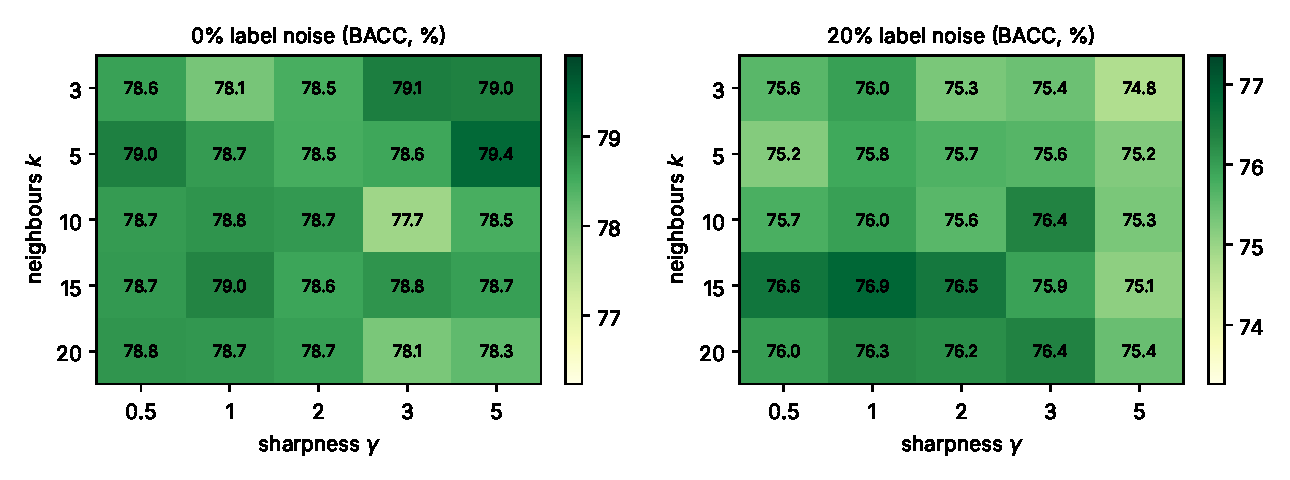
\includegraphics[width=\textwidth]{figures/sensitivity.pdf}
\caption{Sensitivity of the linear \RF{} to the number of voting neighbours $k$ and the sharpness $\gamma$: average BACC over 21 datasets under CV tuning.}
\label{fig:sensitivity}
\end{figure}

%% ---------------------------------------------------------------------------
\section{Discussion}
\label{sec:discussion}

\paragraph{The tuning protocol changes the ranking} Under test-set tuning the three granular-ball least squares models have the three best average ranks among the linear models and the point-based SVM and LSTSVM are near the bottom, in line with the results reported for GBLSTSVM \cite{tanveer2024gblstsvm}. Under CV tuning on the same splits, GBLSTSVM is below LSTSVM at every noise level, by 1.1 to 3.0 points of ACC, and below SVM by 1.4 to 8.1 points. A plausible reason is that the granular-ball models have more hyperparameters, and some of them (the number of clusters per split) change the training set itself, so their best-case score over a grid is further above what cross-validation can find. We therefore recommend that granular-ball classifiers be reported under cross-validation, at least in addition to test-set tuning. For \RF{} the two protocols agree on the comparison with the other granular-ball models, and they disagree on the comparison with SVM on clean data.

\paragraph{Where the proposed model helps and where it does not} The membership is designed for label noise, and this is where the gains are: the advantage of \RF{} over LS-GBLSTSVM and over the point-based models under CV tuning grows with the noise level. On clean data the membership has little to correct. There, a soft-margin SVM on the samples is the better choice under CV tuning, by 1.8 points of ACC and 3.0 points of BACC with the linear kernel. We also note that under test-set tuning the grid of \RF{} is four times as large as that of LS-GBLSTSVM because of $k$ and $\gamma$, which favours \RF{} in that protocol; the CV results are not affected by this, since a larger grid is no advantage when the settings are chosen without the test labels.

\paragraph{GBSVM solved exactly} GBSVM is the weakest model in our tables under both protocols. We checked the solver: with all radii set to zero it reproduces the linear SVM. With the radii, the constraint in \eqref{eq:gbsvm} asks each ball to be at distance $r_j$ beyond the margin, and on several datasets the optimum is $w=0$, which assigns every sample to one class. The published GBSVM results were obtained with particle swarm optimisation, which does not need to reach this optimum. This behaviour of the exact solution deserves a separate study.

\paragraph{Limitations} The experiments cover small and medium datasets with up to 1484 samples. We have not yet run large-scale experiments such as the NDC datasets used in \cite{tanveer2024gblstsvm}; the present implementation computes all pairwise gaps, which is quadratic in the number of balls, and a neighbour search with a spatial index is needed first. The noise in our experiments is uniform label flipping; feature noise and class-dependent label noise were not studied. The diagnostic and sensitivity analyses use 21 of the 35 datasets.

%% ---------------------------------------------------------------------------
\section{Conclusion}
\label{sec:conclusion}

The deletion of single-sample balls in GBLSTSVM removes most mislabelled samples, but also more than half of the correctly labelled ones at 20\% label noise. We proposed to keep all balls and to weight each ball by a radius-aware fuzzy membership: a vote among the balls with the smallest surface gap, weighted by ball size and by the gap. The resulting model, \RF{}, is still trained by solving two linear systems. On 35 datasets it is the best of seven models under test-set tuning at every noise level, with the linear and the Gaussian kernel. Under cross-validation it is the best granular-ball model, and the best linear model overall in ACC from 15\% label noise upwards, while SVM remains better on clean data. Future work includes a faster neighbour search for large-scale data, other noise models, and the use of the membership in other granular-ball classifiers.

\section*{Code availability}
The code and the result files of all experiments are available at \url{https://github.com/Jayagna/GBLSTSVM}.

\appendix
\section{Per-dataset results}
\label{app:per-dataset}

Tables~\ref{tab:per-oracle-0} to \ref{tab:per-cv-20} give the ACC of the linear models on every dataset at 0\% and 20\% label noise under both tuning protocols.

\begin{table}[!p]
\centering
\caption{ACC (\%) on every dataset, linear kernel, test-set tuning, 0\% label noise (mean over 10 splits).}
\label{tab:per-oracle-0}
\scriptsize
\resizebox{\textwidth}{!}{%
\begin{tabular}{lccccccc}
\toprule
Dataset & SVM & TSVM & GBSVM & LSTSVM & GBLSTSVM & LS-GBLSTSVM & \textbf{RF-GBLSTSVM} \\
\midrule
abalone9-18 & 95.91 & 96.86 & 95.36 & 96.36 & 96.95 & 96.91 & \textbf{97.00} \\
brwisconsin & 97.66 & 96.98 & \textbf{98.10} & 97.76 & 97.80 & 97.95 & 97.90 \\
bupa or liver-disorders & 68.27 & 67.60 & 57.69 & 68.27 & \textbf{70.00} & 69.52 & 68.85 \\
cleve & 84.44 & 85.78 & 79.11 & 84.56 & 85.22 & 86.33 & \textbf{86.78} \\
ecoli-0-1-4-6\_vs\_5 & 97.14 & 96.19 & 97.86 & 96.55 & 96.90 & 97.74 & \textbf{98.33} \\
ecoli-0-1-4-7\_vs\_2-3-5-6 & 96.53 & 97.13 & 96.73 & 96.04 & 97.52 & 97.62 & \textbf{97.72} \\
ecoli-0-1\_vs\_5 & 98.61 & 98.06 & 99.17 & 97.36 & 98.75 & 99.03 & \textbf{99.44} \\
ecoli2 & 92.97 & 92.87 & 93.07 & 92.28 & 94.06 & \textbf{94.65} & 94.55 \\
ecoli3 & 92.97 & 92.87 & 93.07 & 92.28 & 94.06 & \textbf{94.65} & 94.55 \\
ecoli4 & 99.31 & 98.22 & 99.01 & 98.71 & 99.21 & 99.41 & \textbf{99.50} \\
fertility & 86.67 & 86.67 & 86.67 & 86.67 & 83.33 & 87.50 & \textbf{90.33} \\
ger & 77.70 & 77.87 & 70.00 & 77.30 & 76.57 & 77.13 & \textbf{78.57} \\
glass2 & 92.31 & 92.77 & 92.31 & 92.46 & 92.15 & 93.54 & \textbf{94.46} \\
glass4 & 96.15 & 96.15 & 95.54 & 96.00 & 94.77 & 97.54 & \textbf{98.31} \\
glass5 & \textbf{98.92} & 91.38 & 95.38 & 96.31 & 95.69 & 97.69 & 98.00 \\
haberman & 76.85 & 77.28 & 75.98 & 77.17 & 77.83 & \textbf{78.26} & 77.93 \\
heart-stat & 85.80 & 87.28 & 77.78 & 86.30 & 87.04 & 87.53 & \textbf{88.02} \\
iono & 89.62 & 87.92 & 64.15 & 88.68 & 79.34 & 90.19 & \textbf{90.57} \\
led7digit-0-2-4-5-6-7-8-9\_vs\_1 & 96.17 & 96.99 & 97.14 & 94.59 & 96.92 & 96.99 & \textbf{97.22} \\
monk2 & 65.75 & 65.75 & 65.75 & 65.75 & 66.35 & 66.35 & \textbf{67.79} \\
monk3 & 50.54 & \textbf{55.63} & 52.34 & 50.54 & 54.91 & 54.73 & 52.10 \\
new-thyroid1 & 98.92 & 96.00 & 99.23 & 98.00 & 98.46 & 99.54 & \textbf{100.00} \\
pima & 77.10 & 77.36 & 74.94 & 77.23 & 78.05 & \textbf{78.53} & 78.27 \\
sonar & 80.48 & 81.11 & 53.97 & 78.89 & 76.35 & 83.02 & \textbf{84.60} \\
transfusion & 77.11 & 79.38 & 78.22 & 78.80 & 79.51 & 79.91 & \textbf{80.84} \\
vehicle 1 & 81.14 & 82.32 & 74.41 & 81.65 & 82.01 & 81.89 & \textbf{82.99} \\
vehicle2 & 97.36 & \textbf{97.87} & 74.41 & 97.24 & 97.13 & 97.09 & 97.83 \\
wdbc & 97.43 & 96.73 & 93.27 & 97.02 & 90.12 & 97.60 & \textbf{98.19} \\
wpbc & 82.37 & 80.51 & 76.95 & 83.05 & 75.08 & 81.86 & \textbf{84.92} \\
yeast-0-2-5-6\_vs\_3-7-8-9 & 92.58 & 93.84 & 92.65 & 92.88 & 93.68 & 93.87 & \textbf{94.17} \\
yeast-0-2-5-7-9\_vs\_3-6-8 & 96.99 & 97.45 & 97.25 & 95.86 & \textbf{97.72} & 97.68 & 97.52 \\
yeast-0-5-6-7-9\_vs\_4 & 92.39 & 93.90 & 91.70 & 91.82 & 93.33 & 93.46 & \textbf{94.03} \\
yeast-2\_vs\_4 & 96.26 & 97.16 & 96.39 & 95.23 & 96.71 & 96.97 & \textbf{97.74} \\
yeast1vs7 & 93.48 & 94.13 & 94.13 & 94.28 & 94.57 & 95.00 & \textbf{95.22} \\
yeast3 & 94.60 & 94.75 & 93.72 & 93.61 & 94.80 & 94.93 & \textbf{95.11} \\
\bottomrule
\end{tabular}}
\end{table}

\begin{table}[!p]
\centering
\caption{ACC (\%) on every dataset, linear kernel, test-set tuning, 20\% label noise (mean over 10 splits).}
\label{tab:per-oracle-20}
\scriptsize
\resizebox{\textwidth}{!}{%
\begin{tabular}{lccccccc}
\toprule
Dataset & SVM & TSVM & GBSVM & LSTSVM & GBLSTSVM & LS-GBLSTSVM & \textbf{RF-GBLSTSVM} \\
\midrule
abalone9-18 & 94.41 & 95.86 & 94.32 & 95.73 & \textbf{96.41} & 96.27 & 96.36 \\
brwisconsin & 96.88 & 97.32 & \textbf{98.05} & 97.02 & 97.46 & \textbf{98.05} & 98.00 \\
bupa or liver-disorders & 66.92 & 64.52 & 57.88 & 65.67 & 71.15 & \textbf{71.25} & 68.27 \\
cleve & 82.56 & 81.67 & 78.22 & 79.56 & 81.33 & 84.44 & \textbf{85.78} \\
ecoli-0-1-4-6\_vs\_5 & 93.69 & 95.95 & 96.67 & 96.07 & 97.26 & 97.26 & \textbf{97.50} \\
ecoli-0-1-4-7\_vs\_2-3-5-6 & 92.87 & 94.55 & 94.85 & 94.55 & 96.73 & \textbf{97.03} & 96.93 \\
ecoli-0-1\_vs\_5 & 94.44 & 96.67 & 98.06 & 96.67 & 97.78 & 98.47 & \textbf{98.89} \\
ecoli2 & 89.11 & 92.67 & 90.79 & 92.08 & 93.86 & 93.96 & \textbf{94.75} \\
ecoli3 & 89.11 & 92.67 & 90.79 & 92.08 & 93.86 & 93.96 & \textbf{94.75} \\
ecoli4 & 95.35 & 97.33 & 98.61 & 97.13 & 98.32 & 98.61 & \textbf{99.01} \\
fertility & 86.67 & 86.67 & 86.67 & 86.67 & 80.00 & 85.33 & \textbf{87.33} \\
ger & 75.13 & 75.57 & 70.00 & 75.50 & 74.97 & 75.37 & \textbf{76.50} \\
glass2 & 92.31 & 92.46 & 92.31 & 92.31 & 93.08 & 93.38 & \textbf{94.00} \\
glass4 & 94.62 & 96.46 & 95.54 & 96.00 & 96.00 & 97.54 & \textbf{98.46} \\
glass5 & 95.38 & 95.69 & 95.38 & 95.69 & 95.54 & \textbf{97.08} & 96.77 \\
haberman & 76.20 & 76.30 & 75.11 & 76.09 & \textbf{78.26} & 78.15 & 77.39 \\
heart-stat & 84.57 & 83.46 & 76.42 & 82.10 & 81.48 & 86.42 & \textbf{87.41} \\
iono & 86.23 & 85.47 & 64.15 & 85.09 & 76.23 & 87.92 & \textbf{88.68} \\
led7digit-0-2-4-5-6-7-8-9\_vs\_1 & 91.73 & 93.31 & 94.06 & 93.83 & 95.34 & \textbf{96.54} & 96.24 \\
monk2 & 65.75 & 65.75 & 65.75 & 66.02 & 66.69 & 66.57 & \textbf{67.57} \\
monk3 & 51.14 & \textbf{54.13} & 51.98 & 51.32 & 53.47 & 53.41 & 52.63 \\
new-thyroid1 & 95.69 & 96.62 & 98.77 & 95.69 & 99.08 & \textbf{100.00} & 99.69 \\
pima & 76.71 & 76.67 & 71.21 & 76.41 & 77.49 & 77.49 & \textbf{77.84} \\
sonar & 72.06 & 72.38 & 53.97 & 71.27 & 72.22 & 78.25 & \textbf{79.37} \\
transfusion & 76.31 & 77.69 & 76.18 & 78.22 & 78.84 & 78.98 & \textbf{79.87} \\
vehicle 1 & 79.61 & 80.04 & 74.41 & 80.67 & 81.34 & 81.14 & \textbf{81.77} \\
vehicle2 & 96.38 & 95.35 & 75.20 & 94.49 & 95.31 & 95.67 & \textbf{96.42} \\
wdbc & 95.79 & 93.63 & 95.09 & 92.87 & 90.23 & \textbf{96.55} & 96.37 \\
wpbc & 77.97 & 77.29 & 76.95 & 78.31 & 69.49 & 79.32 & \textbf{82.03} \\
yeast-0-2-5-6\_vs\_3-7-8-9 & 91.13 & 92.55 & 90.56 & 92.52 & 92.95 & 93.01 & \textbf{93.74} \\
yeast-0-2-5-7-9\_vs\_3-6-8 & 92.62 & 96.56 & 92.62 & 95.99 & 96.95 & \textbf{97.32} & \textbf{97.32} \\
yeast-0-5-6-7-9\_vs\_4 & 90.57 & 91.64 & 90.69 & 91.51 & 92.64 & 92.45 & \textbf{93.14} \\
yeast-2\_vs\_4 & 93.68 & 94.58 & 94.39 & 94.71 & 96.26 & 96.19 & \textbf{96.90} \\
yeast1vs7 & 93.48 & 93.77 & 93.55 & 93.91 & 94.86 & 94.93 & \textbf{95.00} \\
yeast3 & 89.01 & 94.19 & 89.64 & 94.08 & 94.35 & 94.64 & \textbf{95.02} \\
\bottomrule
\end{tabular}}
\end{table}

\begin{table}[!p]
\centering
\caption{ACC (\%) on every dataset, linear kernel, cross-validated tuning, 0\% label noise (mean over 10 splits).}
\label{tab:per-cv-0}
\scriptsize
\resizebox{\textwidth}{!}{%
\begin{tabular}{lccccccc}
\toprule
Dataset & SVM & TSVM & GBSVM & LSTSVM & GBLSTSVM & LS-GBLSTSVM & \textbf{RF-GBLSTSVM} \\
\midrule
abalone9-18 & 88.73 & 89.05 & 71.91 & \textbf{92.73} & 92.50 & 91.59 & 85.50 \\
brwisconsin & 96.93 & 96.44 & \textbf{97.32} & 97.07 & 93.66 & 96.05 & 90.54 \\
bupa or liver-disorders & \textbf{65.96} & 62.79 & 47.31 & 63.85 & 60.10 & 62.21 & 64.04 \\
cleve & \textbf{83.56} & 82.11 & 61.11 & 83.11 & 77.00 & 82.89 & 81.78 \\
ecoli-0-1-4-6\_vs\_5 & 93.81 & \textbf{94.64} & 81.90 & 94.05 & 90.36 & 90.95 & 90.83 \\
ecoli-0-1-4-7\_vs\_2-3-5-6 & 90.30 & 90.69 & 89.01 & 90.69 & \textbf{92.18} & 90.69 & 91.19 \\
ecoli-0-1\_vs\_5 & \textbf{94.86} & 94.03 & 92.22 & 91.39 & 88.19 & 88.47 & 92.78 \\
ecoli2 & 86.24 & \textbf{87.62} & 82.08 & 85.15 & 79.41 & \textbf{87.62} & 82.87 \\
ecoli3 & 86.24 & \textbf{87.62} & 82.08 & 85.15 & 79.41 & \textbf{87.62} & 82.87 \\
ecoli4 & 94.65 & \textbf{97.23} & 96.93 & 96.14 & 94.75 & 96.04 & 95.74 \\
fertility & 68.33 & 64.67 & \textbf{83.75} & 55.33 & 72.86 & 77.50 & 67.00 \\
ger & 70.97 & 68.33 & 70.00 & 69.00 & 68.77 & 69.43 & \textbf{73.40} \\
glass2 & \textbf{82.92} & 74.92 & 26.92 & 76.62 & 74.23 & 79.23 & 76.00 \\
glass4 & \textbf{92.15} & 88.46 & 46.31 & 85.85 & 76.15 & 81.23 & 85.08 \\
glass5 & \textbf{97.08} & 87.23 & 40.77 & 83.54 & 51.45 & 78.46 & 81.85 \\
haberman & \textbf{72.28} & 68.48 & 56.85 & 71.85 & 67.83 & 70.22 & 67.72 \\
heart-stat & \textbf{84.07} & 80.49 & 59.51 & 82.84 & 75.68 & 80.86 & \textbf{84.07} \\
iono & \textbf{86.42} & 85.00 & 58.49 & 79.91 & 70.00 & 84.81 & 83.96 \\
led7digit-0-2-4-5-6-7-8-9\_vs\_1 & 91.43 & 93.68 & 92.26 & 87.22 & 93.98 & 93.98 & \textbf{95.49} \\
monk2 & 55.64 & 48.56 & \textbf{65.75} & 47.24 & 51.10 & 51.38 & 53.81 \\
monk3 & 48.98 & \textbf{50.12} & 48.20 & 48.86 & 50.00 & 49.58 & 48.50 \\
new-thyroid1 & \textbf{97.38} & 95.54 & 96.77 & 96.15 & 92.31 & 96.31 & 96.62 \\
pima & 73.98 & 73.33 & 63.03 & 73.85 & \textbf{74.37} & 74.20 & 74.11 \\
sonar & \textbf{77.46} & 73.02 & 51.59 & 70.16 & 72.22 & 75.24 & 73.17 \\
transfusion & 64.76 & 67.07 & \textbf{69.91} & 67.02 & 67.82 & 69.11 & 69.51 \\
vehicle 1 & \textbf{77.52} & 77.13 & 37.44 & 76.42 & 70.91 & 75.28 & 75.94 \\
vehicle2 & 96.54 & \textbf{96.57} & 74.41 & 96.02 & 92.60 & 95.35 & 95.08 \\
wdbc & \textbf{96.26} & 95.44 & 75.61 & 95.32 & 78.19 & 95.91 & 95.96 \\
wpbc & \textbf{73.56} & 70.17 & 42.03 & 65.76 & 63.84 & 65.59 & 69.32 \\
yeast-0-2-5-6\_vs\_3-7-8-9 & 87.28 & 89.11 & 87.19 & \textbf{89.24} & 86.79 & 88.41 & 88.94 \\
yeast-0-2-5-7-9\_vs\_3-6-8 & 92.88 & \textbf{94.37} & 85.46 & 93.91 & 92.98 & 92.65 & 91.92 \\
yeast-0-5-6-7-9\_vs\_4 & 82.70 & 84.53 & 67.92 & 85.28 & 80.31 & 82.08 & \textbf{88.18} \\
yeast-2\_vs\_4 & 92.06 & 91.48 & 68.19 & 91.55 & 89.10 & \textbf{92.26} & 90.84 \\
yeast1vs7 & 79.20 & 79.49 & 57.32 & 78.62 & \textbf{86.38} & 78.99 & 77.90 \\
yeast3 & 89.46 & 87.65 & 72.13 & 88.54 & \textbf{90.65} & 78.45 & 86.43 \\
\bottomrule
\end{tabular}}
\end{table}

\begin{table}[!p]
\centering
\caption{ACC (\%) on every dataset, linear kernel, cross-validated tuning, 20\% label noise (mean over 10 splits).}
\label{tab:per-cv-20}
\scriptsize
\resizebox{\textwidth}{!}{%
\begin{tabular}{lccccccc}
\toprule
Dataset & SVM & TSVM & GBSVM & LSTSVM & GBLSTSVM & LS-GBLSTSVM & \textbf{RF-GBLSTSVM} \\
\midrule
abalone9-18 & 73.23 & 82.23 & 34.64 & 75.95 & 70.27 & 69.00 & \textbf{89.18} \\
brwisconsin & 96.54 & 96.59 & \textbf{97.41} & 96.63 & 94.05 & 96.59 & 96.88 \\
bupa or liver-disorders & \textbf{61.54} & 61.35 & 49.81 & 61.15 & 60.00 & 60.48 & 57.21 \\
cleve & 78.67 & 77.67 & 73.89 & 76.78 & 71.33 & 79.22 & \textbf{80.44} \\
ecoli-0-1-4-6\_vs\_5 & 76.55 & 86.79 & 82.50 & \textbf{91.19} & 75.48 & 81.90 & 89.76 \\
ecoli-0-1-4-7\_vs\_2-3-5-6 & 74.75 & 80.20 & 66.24 & 76.53 & 65.90 & 82.67 & \textbf{90.20} \\
ecoli-0-1\_vs\_5 & 79.72 & 81.39 & 81.94 & 68.47 & 74.38 & 82.92 & \textbf{89.44} \\
ecoli2 & 74.16 & 73.37 & 63.66 & 80.50 & 72.77 & 67.62 & \textbf{80.59} \\
ecoli3 & 74.16 & 73.37 & 63.66 & 80.50 & 72.77 & 67.62 & \textbf{80.59} \\
ecoli4 & 83.27 & 82.87 & 73.66 & 83.37 & 72.48 & \textbf{88.42} & 85.64 \\
fertility & \textbf{70.67} & 46.67 & 63.33 & 39.00 & 66.67 & 70.00 & 60.33 \\
ger & 68.30 & 68.67 & 70.00 & 69.30 & 62.57 & 68.30 & \textbf{71.90} \\
glass2 & 53.38 & 56.31 & 39.69 & 64.15 & \textbf{67.85} & 58.15 & 48.62 \\
glass4 & \textbf{81.69} & 66.15 & 65.85 & 60.46 & 69.54 & 77.69 & 79.08 \\
glass5 & 63.38 & 51.08 & 53.23 & 62.15 & 65.47 & \textbf{71.08} & 66.77 \\
haberman & 67.39 & 61.74 & 55.87 & 61.74 & 61.74 & 64.78 & \textbf{68.26} \\
heart-stat & \textbf{82.72} & 79.14 & 57.90 & 80.62 & 69.51 & 78.89 & 80.99 \\
iono & \textbf{83.77} & 81.60 & 44.34 & 81.60 & 66.79 & 81.42 & 80.47 \\
led7digit-0-2-4-5-6-7-8-9\_vs\_1 & 74.81 & 78.35 & 69.10 & 73.76 & 62.63 & 77.29 & \textbf{83.61} \\
monk2 & 59.34 & 50.06 & 45.75 & 52.87 & 49.67 & 57.46 & \textbf{61.44} \\
monk3 & 48.56 & \textbf{49.94} & 48.32 & 47.54 & 48.86 & 48.50 & 48.62 \\
new-thyroid1 & 91.85 & 92.15 & \textbf{95.08} & 93.23 & 82.77 & 92.77 & 93.85 \\
pima & 73.33 & 72.34 & 61.65 & 72.47 & 72.77 & 72.86 & \textbf{73.77} \\
sonar & \textbf{66.83} & 62.54 & 53.17 & 62.86 & 63.33 & 62.86 & 61.90 \\
transfusion & 59.56 & 66.44 & 55.20 & 63.91 & 68.09 & 68.49 & \textbf{72.13} \\
vehicle 1 & 74.02 & 73.98 & 43.11 & 71.89 & 67.32 & 71.18 & \textbf{74.61} \\
vehicle2 & \textbf{94.80} & 91.69 & 38.11 & 92.13 & 91.57 & 90.79 & 92.99 \\
wdbc & \textbf{95.38} & 90.99 & 93.22 & 92.05 & 82.28 & 94.04 & 93.57 \\
wpbc & \textbf{63.22} & 55.76 & 48.47 & 55.25 & 58.05 & 59.32 & 61.86 \\
yeast-0-2-5-6\_vs\_3-7-8-9 & 79.47 & 82.09 & 80.46 & 83.41 & 81.39 & 83.28 & \textbf{90.33} \\
yeast-0-2-5-7-9\_vs\_3-6-8 & 77.28 & 87.81 & 84.34 & 88.64 & 86.75 & 89.93 & \textbf{90.79} \\
yeast-0-5-6-7-9\_vs\_4 & 73.46 & 73.27 & 44.09 & \textbf{78.11} & 70.38 & 73.21 & 74.09 \\
yeast-2\_vs\_4 & 84.84 & 88.32 & 62.32 & 87.61 & 77.35 & 85.61 & \textbf{90.84} \\
yeast1vs7 & 62.83 & 48.62 & 30.72 & 56.01 & 59.06 & 68.91 & \textbf{73.91} \\
yeast3 & 81.35 & 88.34 & 53.23 & 89.17 & 85.22 & 86.26 & \textbf{92.62} \\
\bottomrule
\end{tabular}}
\end{table}


\clearpage
\bibliographystyle{elsarticle-num}
\bibliography{refs}

\end{document}
